\documentclass[12pt]{article}
\usepackage{graphicx}
\usepackage{amsmath}
\usepackage{siunitx}
\graphicspath{{images/}}


\title{\huge{Sensors, Measurements \& Instrumentation}}
\author{\huge{Papa Kofi Boahen}}
\date{\today} 

\begin{document}
	\maketitle
	\huge{Roll Number: 10211100334} \par BSc Computer Engineering
	
\section*{Question 1}
Resistance of galvanometer, $R_{G} = \qty{5}{\ohm}$ 
\\ Current through galvanometer, $I_{G} = \qty{15e-3}{\ampere}$
\\ Current through shunt resistor, $I_{R_{sh}}$
\\ Voltage across galvanometer, $V_{G}$
\\ Voltage across shunt resistor, $V_{sh}$
\\ Voltage across multiplier resistor, $V_{M}$
\\ Resistance of shunt, $R_{sh}$
\\ Resistance of multiplier, $R_{M}$


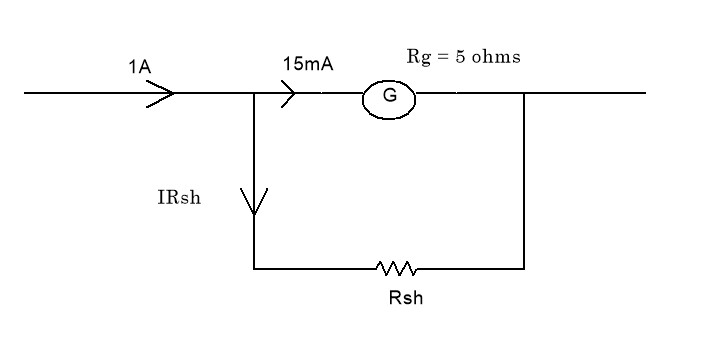
\includegraphics[width=\textwidth]{ques1i}
\begin{align*}
 I) \qquad		I_{R_{sh}} &= 1 -(\num{15e-3})\\
 		I_{R_{sh}} &= \qty{0.985}{\ampere}
\end{align*}

\begin{align*}
     V_G &= V_{sh} \\
     I_G R_G &= I_{R_{sh}} R_{sh} \\ 
     R_{sh} &= \frac{I_{G} R_{G}}{I_{R_{sh}}} \\
     &= \frac{\num{15e-3}\times 5}{\num{0.985}} \\
     &=\underline{\underline{\qty{0.076}{\ohm}}} \\
\end{align*}

Total voltage through multiplier and galvanometer, $V$ \\
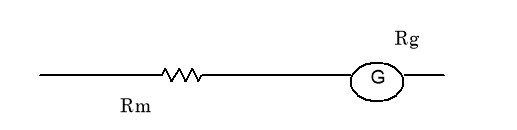
\includegraphics[width=\textwidth]{ques1ii}
\begin{align*}
	II) \qquad V &= V_{M} + V_{G} \\
	           V &= I_{G} R_{M} + I_{G} R_{G} \\
	       R_M &= \frac{V - I_G R_G}{I_G} \\
	      R_M &= \frac{15 -(\num{15e-3}) \times (\num{5}) }{(\num{15e-3})} \\
	      R_M &= \underline{\underline{\qty{995}{\ohm}}} 
\end{align*}

\vspace{1cm}
\section*{Question 2}
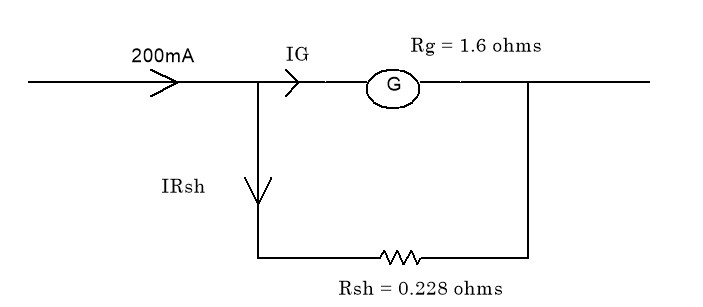
\includegraphics[width=\textwidth]{ques2}
\begin{align*}
\qquad	V_G &= V_{R_{sh}}  \qquad I_{R_{sh}} = 0.2 - I_{G} \\
		I_G R_G &= I_{R_{sh}} R_{sh}    \\
		I_G R_G &= 0.2 R_{sh} - I_G R_{sh} \\
	I_G R_G + I_G R_{sh} &= \num{0.2} R_{sh} \\
	I_G &= \frac{0.2R_{sh}}{R_G + R_{sh}} \\
	   &= \frac{\num{0.2} \times \num{0.228}}{\num{1.6} + \num{0.228}} \\
	   &= 0.0249 \\
	   &= \underline{\underline{\qty{24.9}{\milli\ampere}}}
\end{align*}

\vspace{1cm}
\section*{Question 3}
\begin{figure}[h]
	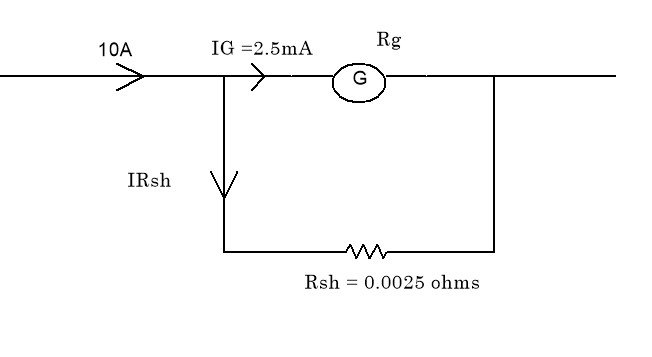
\includegraphics[width=\textwidth]{ques3}
	\centering
\end{figure}
\begin{align*}
	I_{R_{sh}} &= \num{10} - (\num{2.5e-3}) \\
	I_G R_G &= I_{R_{sh}} R_{sh} \\
	R_G &= \frac{\num{9.9975} \times \num{0.0025}}{\num{2.5e-3}} \\
		&= \underline{\underline{\qty{9.9975}{\ohm}}}
\end{align*}

\vspace{1cm}
\section*{Question 4}
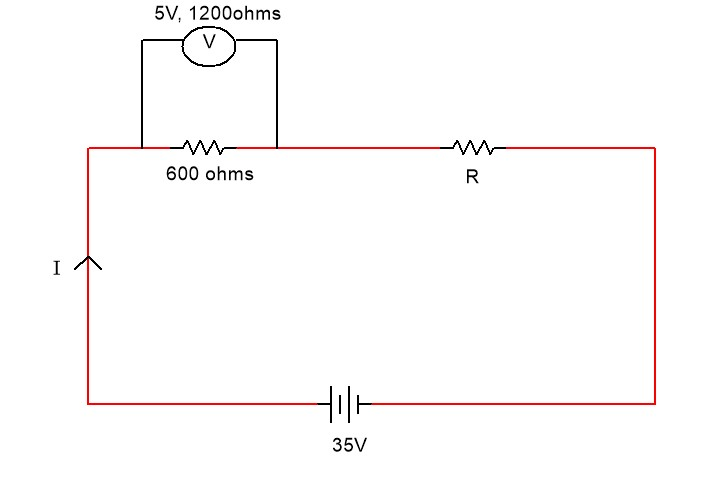
\includegraphics[width=\textwidth]{ques4} \\
 Resistance \ across \ parallel \ connection 
\begin{align*}
\noindent R_{\|} &= \frac{1200 \times 600}{1200 + 600} \\
	&= 400 \Omega
\end{align*}

\begin{align*}
	V &=I R_{\|} \\
	I &= \frac{V}{R_{\|}} \\
	&= \frac{5}{400} \\
	&= \frac{1}{80} \ A
\end{align*}


\begin{align*}
	Voltage \ across \ R: 35-5 = \qty{30}{\volt} \\	
		R=\frac{V}{I} &=\frac{30}{1 / 80} \\
		&= \underline{\underline{2400 \Omega}}
\end{align*}


\end{document}


